%! suppress = EscapeHashOutsideCommand
%! suppress = Quote
%! suppress = MissingImport
%! suppress = MissingLabel
%! suppress = LineBreak

% CLI args https://tex.stackexchange.com/a/1501
\newif\ifhandout
\input{flags}

%! suppress = MissingLabel
%! suppress = DocumentclassNotInRoot
%! suppress = DiscouragedUseOfDef

% * Make friends tikz & colors
%   https://en.wikibooks.org/wiki/LaTeX/Colors
% * To enable vertical top alignment globally
%   https://tex.stackexchange.com/questions/9889/positioning-content-at-the-top-of-a-beamer-slide-by-default
% * Set handout from CLI
%   https://tex.stackexchange.com/a/1501
\ifhandout
\documentclass[usenames, dvipsnames, handout]{beamer} % https://tex.stackexchange.com/questions/224091/beamer-how-to-disable-pause-temporarily
\else
\documentclass[usenames, dvipsnames]{beamer}
\fi
% ------------------------------------------------

% Graphics
\usepackage{color}
\usepackage{tabularx}
\usepackage{tikz}
% https://tikz.dev/tikz-graphs
\usetikzlibrary{positioning, shapes.geometric, arrows, automata, graphs}
\tikzset{
    expr/.style={ellipse, draw=gray!60, fill=gray!5, very thick, minimum size=7mm, yshift=0.7cm},
    hexpr/.style={ellipse, draw=gray!60, fill=blue!15, very thick, minimum size=7mm, yshift=0.7cm},
    stmt/.style={rectangle, draw=gray!60, fill=gray!5, very thick, minimum size=5mm, yshift=0.7cm},
    decl/.style={rectangle, draw=blue!60, fill=gray!5, very thick, minimum size=5mm, yshift=0.7cm},
    hdecl/.style={rectangle, draw=blue!60, fill=blue!15, very thick, minimum size=5mm, yshift=0.7cm},
    subtree/.style={shape border rotate=90, isosceles triangle, draw=gray!60, fill=gray!5, very thick, minimum size=5mm, yshift=0.0cm},
}
\usepackage{blkarray}
\usepackage{graphicx}
\usepackage{forest} % https://tex.stackexchange.com/questions/198405/how-to-change-the-color-of-subtrees-in-tikz-qtree
% ------------------------------------------------

% Math
\usepackage{amsmath, amsfonts}
\usepackage{amssymb}
\usepackage{proof}
\usepackage{mathrsfs}
% Crossed-out symbols
% https://tex.stackexchange.com/questions/75525/how-to-write-crossed-out-math-in-latex
\usepackage[makeroom]{cancel}
\usepackage{mathtools}
% ------------------------------------------------

% Additional font sizes
% https://www.overleaf.com/learn/latex/Questions/How_do_I_adjust_the_font_size%3F
\usepackage{moresize}
% Additional colors
% https://www.overleaf.com/learn/latex/Using_colours_in_LaTeX
\usepackage{xcolor}
% Textual math symbols
\usepackage{textcomp}
% ------------------------------------------------

% Language
\usepackage[utf8] {inputenc}
\usepackage[T2A] {fontenc}
\usepackage[english, russian] {babel}
\usepackage{indentfirst, verbatim}
\usetikzlibrary{cd, babel}
% ------------------------------------------------

% Fonts: https://sites.math.washington.edu/~reu/docs/latex_symbols.pdf
\usepackage{stmaryrd}
\usepackage{cmbright}
\usepackage{wasysym}
\usepackage[weather]{ifsym} % https://tex.stackexchange.com/questions/100424/how-to-use-the-ifsym-package
% https://tex.stackexchange.com/questions/615300/pdflatex-builtin-glyph-names-is-empty
\pdfmapline{=dictsym DictSym <dictsym.pfb}
\pdfmapline{=pigpen <pigpen.pfa}
\usepackage{dictsym}
% ------------------------------------------------

% Code
% * Needs -shell-escape build flag
%   https://tex.stackexchange.com/questions/99475/how-to-invoke-latex-with-the-shell-escape-flag-in-texstudio-former-texmakerx
% * Set build directory
%   https://tex.stackexchange.com/questions/339931/latex-minted-package-using-custom-output-directory-build
\usepackage{minted}
\setminted{xleftmargin=\parindent, autogobble, escapeinside=\#\#}
% ------------------------------------------------

% Template
\usetheme{CambridgeUS}
\usecolortheme{dolphin}
% https://tex.stackexchange.com/questions/231439/beamer-how-to-make-font-larger-for-page-numbers
\setbeamerfont{headline}{size=\scriptsize}
\setbeamerfont{footline}{size=\scriptsize}
% Remove heddline
% https://tex.stackexchange.com/questions/33146/how-could-i-remove-a-header-in-a-beamer-presentation
%\setbeamertemplate{headline}{}
% Slide sizes
% https://tex.stackexchange.com/questions/56768/how-to-set-a-small-default-font-size-with-beamer
%\geometry{paperwidth=140mm,paperheight=105mm} % 4:3
\geometry{paperwidth=168mm,paperheight=105mm} % 16:10
% Remove navigation bar
% https://stackoverflow.com/questions/3210205/how-to-get-rid-of-navigation-bars-in-beamer
\beamertemplatenavigationsymbolsempty
% ------------------------------------------------

% Bullets
% https://9to5science.com/change-bullet-style-formatting-in-beamer
% https://tex.stackexchange.com/questions/185742/i-need-to-change-color-of-beamer-itemize-and-subitem-separately
\setbeamertemplate{itemize item}{\scriptsize\raise1.25pt\hbox{\donotcoloroutermaths$\blacktriangleright$}}
\setbeamertemplate{itemize subitem}{\scriptsize\raise1.5pt\hbox{\donotcoloroutermaths$\blacktriangleright$}}
\setbeamertemplate{itemize subsubitem}{\tiny\raise1.5pt\hbox{\donotcoloroutermaths$\blacktriangleright$}}
\setbeamertemplate{enumerate item}{\insertenumlabel.}
\setbeamertemplate{enumerate subitem}{\insertenumlabel.\insertsubenumlabel}
\setbeamertemplate{enumerate subsubitem}{\insertenumlabel.\insertsubenumlabel.\insertsubsubenumlabel}
% ------------------------------------------------

% Table of contents format
% https://tex.stackexchange.com/questions/642927/format-table-of-contents-in-beamer
\setbeamertemplate{section in toc}{%
        {\color{blue}\inserttocsectionnumber.}
    \inserttocsection\par%
}
\setbeamertemplate{subsection in toc}{%
        {\color{blue}\hspace{1em}\scriptsize\raise1.25pt\hbox{\donotcoloroutermaths$\blacktriangleright$}}
    \inserttocsubsection\par%
}
\setbeamertemplate{subsubsection in toc}{%
        {\color{blue}\hspace{2em}\tiny\raise1.25pt\hbox{\donotcoloroutermaths$\blacktriangleright$}}
    \inserttocsubsubsection\par%
}
% ------------------------------------------------

% Misc
\usepackage{multicol}
\usepackage{hyperref}
\usepackage{soul} % https://tex.stackexchange.com/questions/23711/strikethrough-text
% ------------------------------------------------

% Fix \pause for amsmath package envs (black black magic)
% https://tex.stackexchange.com/questions/16186/equation-numbering-problems-in-amsmath-environments-with-pause/75550#75550
% https://tex.stackexchange.com/questions/6348/problem-with-beamers-pause-in-alignments
%! suppress = Makeatletter
\makeatletter
\let\save@measuring@true\measuring@true
\def\measuring@true{%
    \save@measuring@true
    \def\beamer@sortzero##1{\beamer@ifnextcharospec{\beamer@sortzeroread{##1}}{}}%
    \def\beamer@sortzeroread##1<##2>{}%
    \def\beamer@finalnospec{}%
}
%! suppress = Makeatletter
\makeatother
% ------------------------------------------------

% Sections
\newcommand{\sectionplan}[1]{\section{#1}%
    \begin{frame}[noframenumbering]{Содержание}
        \tableofcontents[currentsection]
    \end{frame}
}
\newcommand{\subsectionplan}[1]{\subsection{#1}%
    \begin{frame}[noframenumbering]{Содержание}
        \tableofcontents[currentsubsection]
    \end{frame}
}
% ------------------------------------------------

% Footnotes
\renewcommand{\thefootnote}{\arabic{footnote}}
\renewcommand{\thempfootnote}{\arabic{mpfootnote}}
% https://tex.stackexchange.com/questions/28465/multiple-footnotes-at-one-point
\usepackage{fnpct}
% ------------------------------------------------

% Links
% Colors also links on slide foot.
%\hypersetup{
%    colorlinks=true,
%    citecolor=blue,
%    linkcolor=blue,
%    urlcolor=blue
%}
% ------------------------------------------------

% Appendix
% Slide numbers
% https://tex.stackexchange.com/questions/70448/dont-count-backup-slides
\usepackage{appendixnumberbeamer}
\newcommand{\backupbegin}{
    \newcounter{framenumbervorappendix}
    \setcounter{framenumbervorappendix}{\value{framenumber}}
}
\newcommand{\backupend}{
    \addtocounter{framenumbervorappendix}{-\value{framenumber}}
    \addtocounter{framenumber}{\value{framenumbervorappendix}}
}
% ------------------------------------------------

% Custom commands
% * Decor
\newcommand{\newtopic}[0]{$+$} % item: new topic on "in previous series"
\newcommand{\then}{$\Rightarrow$} % item: consequences
\newcommand{\pop}[0]{\SunCloud} %item:  general eduation
\newcommand{\popslide}[0]{(\pop)}
\newcommand{\advanced}[0]{$\varhexstar$} % item: advanced science
\newcommand{\advancedslide}[0]{(\advanced)}
\newcommand{\practical}[0]{\dstechnical} % item: practical programming notions
\newcommand{\practicalslide}[0]{(\practical)}
\newcommand{\todo}[0]{todo} % item: question
\newcommand{\answer}[0]{\Lightning} % item: answer to the previous question
\newcommand{\eg}[0]{e.g.} % item: example
\newcommand{\defi}[0]{$\Delta$} % item: definition on smth
\newcommand{\textdefi}[1]{\textbf{#1}}
\newcommand{\positive}{$+$} % item: pros
\newcommand{\negative}{{\color{red} $-$}} % item: cons
\newcommand%! suppress = EscapeHashOutsideCommand
\NB[1][0.3]{N\kern-#1em{B}} % default kern amount: -0.3em
\renewcommand{\emph}[1]{{\color{blue} \textit{#1}}}
\newcommand{\vocab}[1]{\textbf{#1}} % item: important new word
% * Lambda calculi
\newcommand{\comb}[1]{\mathbf{#1}} % defined combinator
\newcommand{\term}[1]{\mathbf{#1}} % predefined lambda-term reference
\newcommand{\termdef}{\coloneqq} % lamda term binding
\newcommand{\step}{\rightsquigarrow} % reduction step
\newcommand{\sstep}{\twoheadrightarrow} % multiple steps reduction
\newcommand{\ap}{~} % lambda-term application
\newcommand{\subst}[3]{\left[#2 \mapsto #3 \right] #1} % substitution
\newcommand{\eqbeta}{=_\beta} % beta equality
\newcommand{\eqeta}{=_\eta} % eta-equality
\newcommand{\eqt}{=} % tree-equality of terms
\newcommand{\tlist}[1]{\term{[}#1\term{]}} % list-term
% * Legacy
%\newcommand{\err}[0]{\textcolor{red}{ошибка}} % compilation error

% ------------------------------------------------

% Speaker notes
% https://tex.stackexchange.com/questions/114219/add-notes-to-latex-beamer
% https://tex.stackexchange.com/questions/35444/split-beamer-notes-across-multiple-notes-pages/35496#35496
%\setbeameroption{show notes on second screen=right} % enable speaker notes
%--------------------------------------

\author[]{Андрей Стоян, Илья Колегов, Дмитрий Халанский}
\institute[MSE ITMO]{MSE ITMO}


\title[12. Трансформеры монад]{Практика 12. Трансформеры монад}
\date{осень 2024}

\begin{document}

    \setcounter{framenumber}{-1}
    \maketitle

    \begin{frame}[fragile]{В предыдущих сериях}
        \begin{itemize}
            \item \mintinline{haskell}|Compose|
            \item Монады, стандартные монады
            \item[\newtopic] Трансформеры монад
        \end{itemize}
    \end{frame}

    \begin{frame}[noframenumbering]{Содержание}
        \tableofcontents
    \end{frame}


    \sectionplan{Recall: monads}

    \begin{frame}[fragile]{Абстрактный тип данных --- \mintinline{haskell}|Monad|}
        \vspace{-0.5em}
        \begin{itemize}
            \item[\defi] АДТ --- интерфейс конструирования обитателей некоторого множества
            \item[\eg] АТД стек: операции \texttt{push(elem)} и \texttt{pop -> elem}
            \item[\eg] АТД \mintinline{haskell}|Monad|: операции \mintinline{haskell}|pure| и \mintinline{haskell}|>>=|
            \item[\eg] Множества: \mintinline{haskell}|[]|, \mintinline{haskell}|Maybe|, \mintinline{haskell}|Either e|
            \item[\eg] Даже множества функций: \mintinline{haskell}|newtype State s a = State (s -> (a, s))|
            \item[\todo] Как следующую функцию сконструировать с помощью \mintinline{haskell}|Monad|?
            \begin{minted}{haskell}
                computation :: s -> (a, s)
                computation s = let s' = f s in (g s, s')
            \end{minted}
            \item[\answer] \pause
            \begin{minted}{haskell}
                computation = runState do
                  s <- get   -- get    ::              s -> (s , s)
                  modify f   -- modify :: (s -> s) -> (s -> ((), s))
                  pure (g s) -- pure   :: a ->        (s -> (a , s))
            \end{minted}
        \end{itemize}
    \end{frame}

    \begin{frame}[fragile]{Вычисления из сложных множеств (доменов)}
        \begin{itemize}
            \item Вычисление с двумя ячейками состояния лежит в \texttt{s -> s' -> ((a, s), s')}
            \item Для этого множества нужно определить все операции АДТ:
            \begin{itemize}
                \item Удобный способ конструирования обитателей: \mintinline{haskell}|Monad|
                \item Функции \mintinline{haskell}|get|, \mintinline{haskell}|put|, \mintinline{haskell}|modify| для \texttt{s}
                \item Те же функции \mintinline{haskell}|get2|, \mintinline{haskell}|put2|, \mintinline{haskell}|modify2| для \texttt{s'}\ldots
            \end{itemize}
            \item[\NB] Приходится переопределять всё каждый раз для новых доменов!
            \item Проблема известна как expression problem, stable denotations, extensible interpreters\footnote{\color{blue} \url{https://okmij.org/ftp/Computation/having-effect.html}.}
        \end{itemize}
    \end{frame}

    \begin{frame}[fragile]{Супер-монады \popslide}
        \begin{itemize}
            \item Можно делать Super Monad сразу со всем необходимым
            \item[\eg] \mintinline{haskell}|newtype Super env err a = Super { runSuper :: env -> IO (Either err a) }|
            \item[\eg] \mintinline{haskell}|newtype Super effs a = Super { runSuper :: IO a }|
            \item[\negative] Медленно работает, не zero-cost abstraction\footnote{Zero-cost не значит бесплатно, а значит --- если не используешь, то не платишь за её присутствие.}
            \item[\negative] Не модульно --- сложно поддерживать и использовать частями
            \item[\negative] Не получится легко подменять реализации и домены
        \end{itemize}
    \end{frame}

    \begin{frame}[fragile]{Монады не композируются \popslide}
        \vspace{-0.5em}
        \begin{itemize}
            \item \mintinline{haskell}|join :: (Monad m, Monad n) => Compose m n (Compose m n a) -> Compose m n a|
            \item Запишем без обёрток для наглядности:
            \begin{minted}{haskell}
                join :: (Monad m, Monad n) => m (n (m (n a))) -> m (n a)
            \end{minted}
            \item Можно попробовать переставить \texttt{m} и \texttt{n} местами и свести к двум \texttt{join}
            \item[\NB] Но монады в общем случае не коммутируют
            \item[\eg] Попробуем переставить \mintinline{haskell}|Reader| и \mintinline{haskell}|Writer|
            \begin{itemize}
                \item[1.] \mintinline{haskell}|Reader e (Writer w a)| имеет движок \mintinline{haskell}|e -> (w, a)|
                \item[2.] \mintinline{haskell}|Writer w (Reader e a)| имеет движок \mintinline{haskell}|(w, e -> a)|
                \item[\advanced] Алгебраически видно, что это не изоморфные типы: $(w * a)^e \neq w * a ^ e$
                \item Разумной реализации тоже не получается, перестановка от 1 к 2 теряет лог:
                \begin{minted}{haskell}
                    dist :: Monoid w => (e -> (w, a)) -> (w, e -> a)
                    dist q = (mempty, \e -> fst (q e))
                \end{minted}
            \end{itemize}
        \end{itemize}
    \end{frame}


    \sectionplan{Love. Death. Transformers}

    \begin{frame}[fragile]{Обобщаем до семейства множеств вычислений}
        \begin{itemize}
            \item Программа с одной глобальной переменной задаёт функцию \texttt{s -> (a, s)}
            \item А если глобальных переменных две --- \texttt{s -> s' -> ((a, s), s')}
            \item Оба варианта представимы как частные случаи семейства \texttt{s -> m (a, s)}
            \begin{minted}{haskell}
                newtype StateT s m a = StateT { runStateT :: s -> m (a, s) }
            \end{minted}
            \item[\todo] Выберите подходящие \texttt{m}
            \item[\todo] Реализуйте \mintinline{haskell}|get| и \mintinline{haskell}|put| для \mintinline{haskell}|StateT|
            \item[\todo] Как сконструировать с помощью \mintinline{haskell}|Monad (StateT s m)|?
            \begin{minted}{haskell}
                computation :: s -> (a, s); computation s = let s' = f s in (g s, s')
            \end{minted}
            \item[\answer] \pause Первый: \texttt{m a = Identity a}, второй: \texttt{m a = s' -> (a, s')}
            \item[\answer] \pause
            \begin{minted}{haskell}
                get :: Monad m => StateT s m s; get = StateT \s -> pure (s, s)
            \end{minted}
            \item[\answer] \pause
            \begin{minted}{haskell}
                computation = runIdentity . runStateT do
                  s <- get   -- get    ::              s -> Identity (s , s)
                  modify f   -- modify :: (s -> s) -> (s -> Identity ((), s))
                  pure (g s) -- pure   :: a ->        (s -> Identity (a , s))
            \end{minted}
        \end{itemize}
    \end{frame}

    \begin{frame}[fragile]{Работа с вложенным состоянием}
        \begin{minted}{haskell}
            newtype StateT s m a = StateT { runStateT :: s -> m (a, s) }
        \end{minted}
        \begin{itemize}
            \item[\todo] Реализуйте способ поработать с вложенным состоянием
            \begin{minted}{haskell}
                StateT s' Identity a -> StateT s (StateT s' Identity) a
                (s' -> (a, s'))      -> (s -> s' -> ((a, s), s'))
            \end{minted}
            \item[\todo] Реализуйте для произвольной вложенной монады
            \item[\answer] \pause
            \begin{minted}{haskell}
                liftState :: (s' -> (a, s')) -> (s -> s' -> ((a, s), s'))
                liftState comp = \s -> \s' -> let (x, new) = comp s' in ((x, s), new)
            \end{minted}
            \item[\answer] \pause
            \begin{minted}{haskell}
                liftState :: Monad m => m a -> StateT s m a
                liftState ma = StateT \s -> (,s) <$> ma
            \end{minted}
        \end{itemize}
    \end{frame}

    \begin{frame}[fragile]{Lifting}
        \begin{minted}{haskell}
            newtype StateT s m a = StateT { runStateT :: s -> m (a, s) }
        \end{minted}
        \begin{itemize}
            \item Перегрузим \mintinline{haskell}|lift| по трансформеру с помощью класса типов
            \begin{minted}{haskell}
                class MonadTrans t where
                  lift :: Monad m => m a -> t m a
            \end{minted}
            \item[\todo] Реализуйте \mintinline{haskell}|instance MonadTrans (StateT s)|
            \item[\todo] Сконструируйте в терминах трансформеров следующее вычисление
            \begin{minted}{haskell}
                computation :: Int -> (Int, String)
                computation = \e -> (e + 2, show e ++ show (e + 1))
            \end{minted}
            \item[\answer] \pause
            \begin{minted}{haskell}
                computation = runIdentity . runWriterT . runReaderT do
                  x <- ask; lift (tell $ show x)
                  y <- asks (+ 1); lift (tell $ show y)
                  pure (y + 1)
            \end{minted}
        \end{itemize}
    \end{frame}

    \begin{frame}[fragile]{Неявный lifting (библиотека mtl)}
        \vspace{-0.5em}
        \begin{itemize}
            \item Перегрузим функции стандартных монад по результирующей монаде
            \begin{minted}{haskell}
                class MonadReader e m | m -> e where
                  ask :: m e
            \end{minted}
            \item Для каждого трансформера определим, как в нем должна работать операция
            \begin{minted}{haskell}
                instance MonadReader e m => MonadReader e (StateT s m) where
                  ask = lift ask
            \end{minted}
            \item Можем вообще забыть тип трансформера и требовать от него конкретные свойства
            \begin{minted}{haskell}
                computation :: (MonadReader String m, MonadState Int m) => m a
            \end{minted}
        \end{itemize}
    \end{frame}

    \begin{frame}[fragile]{Анализ трансформеров}
        \begin{center}
            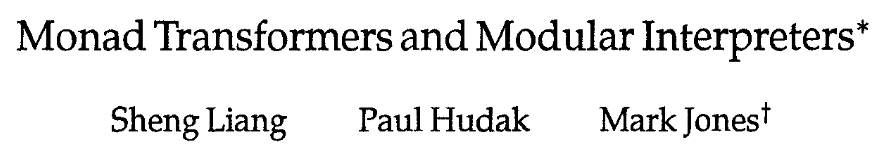
\includegraphics[width=0.5\textwidth]{figs/transformers}
        \end{center}
        \begin{itemize}
            \item[\positive] Позволяют инкрементально и модульно реализовывать функциональность eDSLs
            \item[\positive] Можно делать код полиморфным по стеку трансформеров, требуя интерфейсы
            \item[\negative] Сложны в программировании и изучении (no chances mainstream)
            \item[\negative] Башни существенно замедляют программу, особенно если стек абстрагирован
            \item[\negative] Требуют существенного количества языковых фич для реализации и использования
            \item[\negative] FunDeps ограничивают каждый слой в стеке одним экземпляром
            \item[\negative] Требуют для каждого трансформера реализовать каждый интерфейс
            \item[\negative] Порядок трансформеров играет роль, её можно понять только из реализации трансформера, множество упорядочений бесполезны
        \end{itemize}
    \end{frame}

    \sectionplan{Материалы}

    \begin{frame}[fragile]{Что посмотреть в транспорте}
        \begin{itemize}
            \item \href{https://markkarpov.com/post/the-monads}{\color{blue}(post) The monads of Haskell --- Mark Karpov}
            \item \href{https://youtu.be/m821Vz8N_bo?si=f-2cR0QExCWZr-BK}{\color{blue} [Haskell'23] The Evolution of Effects }
            \item \href{https://youtu.be/qgfCmQ-2tW0?si=6BjvijRPU2hEmk49}{\color{blue}  Keynote: Daniel Spiewak - The Case For Effect Systems }
            \item \href{https://www.youtube.com/live/0jI-AlWEwYI?si=KzgcHDgZ4GseytRA}{\color{blue} Alexis King - ``Effects for Less'' ZuriHac 2020}
            \item \href{https://youtu.be/vfDazZfxlNs?si=Sjfitsfe33jpbMth}{\color{blue}  ``Building Haskell Programs with Fused Effects'' by Patrick Thomson}
        \end{itemize}
    \end{frame}

    \begin{frame}[fragile]{Серьёзные материалы}
        \begin{itemize}
            \item \href{https://okmij.org/ftp/Computation/having-effect.html}{\color{blue} Oleg Kiselyev Blog --- Having an Effect}
            \item \href{https://dl.acm.org/doi/pdf/10.1145/199448.199528}{\color{blue} Liang, S., Hudak, P. and Jones, M., 1995, January. Monad transformers and modular interpreters. In Proceedings of the 22nd ACM SIGPLAN-SIGACT symposium on Principles of programming languages (pp. 333-343).}
            \item \href{https://scholar.google.com/scholar?hl=en&as_sdt=0%2C5&q=Monad+Transformers+and+Modular+Algebraic+Effects&btnG=}{\color{blue}Schrijvers, T., Piróg, M., Wu, N. and Jaskelioff, M., 2019, August. Monad transformers and modular algebraic effects: what binds them together. In Proceedings of the 12th ACM SIGPLAN International Symposium on Haskell (pp. 98-113).}
            \item \href{https://www.youtube.com/playlist?list=PLt7hcIEdZLAkebYy70DdBDm2qLrw7ptfp}{\color{blue}  OPLSS 2018 -- Andrej Bauer -- Algebraic Effects and Handlers}
        \end{itemize}
    \end{frame}

\end{document}
